%----------------------------------------------------------------------------------------
%	PACKAGES AND OTHER DOCUMENT CONFIGURATIONS
%----------------------------------------------------------------------------------------
\documentclass[11pt, a4paper,oneside]{ctexbook}

%----------------------------------------------------------------------------------------
%	TITLE PAGE
%----------------------------------------------------------------------------------------

\newcommand*{\titleGP}{\begingroup % Create the command for including the title page in the document
\centering % Center all text
\vspace*{\baselineskip} % White space at the top of the page

\rule{\textwidth}{1.6pt}\vspace*{-\baselineskip}\vspace*{2pt} % Thick horizontal line
\rule{\textwidth}{0.4pt}\\[\baselineskip] % Thin horizontal line

{\LARGE \textbf{国际教育-小学系列} \\[0.3\baselineskip] \textbf{中文版}}\\[0.2\baselineskip] % Title

\rule{\textwidth}{0.4pt}\vspace*{-\baselineskip}\vspace{3.2pt} % Thin horizontal line
\rule{\textwidth}{1.6pt}\\[\baselineskip] % Thick horizontal line

\scshape % Small caps
\href{https://fieldworkeducation.com/about}{Fieldwork-Education}\\[\baselineskip] % Tagline(s) or further description
\href{https://fieldworkeducation.com/curriculums/primary-years}{IPC}\par % Location and year

\vspace*{4\baselineskip} % Whitespace between location/year and editors

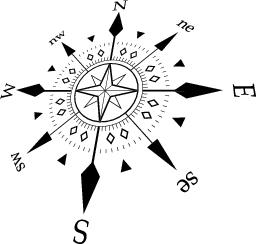
\includegraphics[width=10cm]{compass}


\vfill % Whitespace between editor names and publisher logo

{\itshape2398419426@buaa.edu.cn\par} % Editor list
{\itshape HaotianMichael \par} % Editor affiliation
\vspace*{0.5\baselineskip}
{\scshape 2018} \\ 
{\scshape Powered by \LaTeX \\[0.3\baselineskip]} % Year published

\endgroup}


\usepackage{graphicx} % Required for including pictures
\graphicspath{{Images/}} % Specifies the directory where pictures are stored
\CTEXsetup[format={\Large\bfseries}]{section}    %make section left justifing
%----------------------------------------------------------------------------------------
%       Localization
%----------------------------------------------------------------------------------------
\usepackage[UTF8,adobefonts]{ctex}
\usepackage{array, booktabs}
\usepackage{graphicx}
\usepackage[x11names]{xcolor}
\usepackage{colortbl}
\usepackage{fontspec}
\newcommand{\foo}{\color{baseD}\makebox[0pt]{\textbullet}\hskip-0.5pt\vrule width 1pt\hspace{\labelsep}}

%\setmainfont[Boldont=WenQuanYi Micro Hei]{AR PL SungtiL GB}
%\setsansfont[BoldFont=WenQuanYi Micro Hei]{AR PL KaitiM GB}
%\setmonofont{DejaVu Sans Mono}

%\XeTeXlinebreaklocale "zh"
%\XeTeXlinebreakskip = 0pt plus 1pt minus 0.1pt

\usepackage[top=1in,bottom=1in,left=1.25in,right=1.25in]{geometry}
%\linespread{1.2}

\usepackage[Glenn]{fncychap}

\usepackage{fancyhdr}
\setlength{\headheight}{15.2pt}

%----------------------------------------------------------------------------------------
%       Useful Packages
%----------------------------------------------------------------------------------------
\usepackage{color}
\usepackage{url}
\usepackage[colorlinks, linkcolor=black,anchorcolor=black, citecolor=black]{hyperref}

\usepackage{xcolor} % Required for specifying colors by name
\definecolor{ocre}{RGB}{243,102,25} % Define the orange color used for highlighting throughout the book

% BASE16
\definecolor{base0}{HTML}{181818}
\definecolor{base1}{HTML}{282828}
\definecolor{base2}{HTML}{383838}
\definecolor{base3}{HTML}{585858}
\definecolor{base4}{HTML}{B8B8B8}
\definecolor{base5}{HTML}{D8D8D8}
\definecolor{base6}{HTML}{E8E8E8}
\definecolor{base7}{HTML}{F8F8F8}
\definecolor{base8}{HTML}{AB4642}
\definecolor{base9}{HTML}{DC9656}
\definecolor{baseA}{HTML}{F7CA88}
\definecolor{baseB}{HTML}{A1B56C}
\definecolor{baseC}{HTML}{86C1B9}
\definecolor{baseD}{HTML}{7CAFC2}
\definecolor{baseE}{HTML}{BA8BAF}
\definecolor{baseF}{HTML}{A16946}
\definecolor{Gray}{HTML}{CCCCCC}
\definecolor{linkcolor}{HTML}{EC008C}
\definecolor{codecolorpink}{HTML}{CC00FF}
\definecolor{NoteColorFont}{HTML}{6D727D}
\definecolor{NoteColorLine}{HTML}{C3CAD9}
\definecolor{ExeColorFont}{HTML}{FF9900}
\definecolor{ExeColorLine}{HTML}{FFF678}
\definecolor{ExeColorBack}{HTML}{FFFFCC}
\definecolor{ThinkColorFont}{HTML}{629D81}
\definecolor{ThinkColorLine}{HTML}{93E87D}
\definecolor{ThinkColorBack}{HTML}{C1FA9B}

\usepackage{amsmath,amsfonts,amssymb,amsthm} % For math equations, theorems, symbols, etc
\usepackage{booktabs} % For tables
\usepackage{tabularx}
\usepackage{multirow} % for multiple row tables.
\usepackage{lettrine}    %expand font size 
\usepackage{indentfirst}  %indent at beginning


%\makeatletter
%\renewcommand{\section}{\@startsection{section}{1}{0mm}
%  {-\baselineskip}{0.5\baselineskip}{\bf\leftline}}
%\makeatother


%----------------------------------------------------------------------------------------
%       Some Extra Definitions
%----------------------------------------------------------------------------------------

\RequirePackage[framemethod=default]{mdframed} % Required for creating the theorem, definition, exercise and corollary boxes

% Exercise box
\newmdenv[skipabove=10pt,
skipbelow=10pt,
rightline=false,
leftline=true,
topline=false,
bottomline=false,
backgroundcolor=ExeColorBack,
linecolor=ExeColorLine,
innerleftmargin=5pt,
innerrightmargin=5pt,
innertopmargin=5pt,
innerbottommargin=5pt,
leftmargin=0cm,
rightmargin=0cm,
linewidth=12pt]{eBox}

% Thinking box
\newmdenv[skipabove=10pt,
skipbelow=10pt,
rightline=false,
leftline=true,
topline=false,
bottomline=false,
backgroundcolor=ThinkColorBack!30,
linecolor=ThinkColorLine,
innerleftmargin=5pt,
innerrightmargin=5pt,
innertopmargin=5pt,
innerbottommargin=5pt,
leftmargin=0cm,
rightmargin=0cm,
linewidth=12pt]{tBox}

% Note box
\newmdenv[skipabove=10pt,
skipbelow=10pt,
rightline=false,
leftline=true,
topline=false,
bottomline=false,
backgroundcolor=NoteColorLine!15,
linecolor=NoteColorLine,
innerleftmargin=5pt,
innerrightmargin=5pt,
innertopmargin=5pt,
innerbottommargin=5pt,
leftmargin=0cm,
rightmargin=0cm,
linewidth=12pt]{nBox}

% Boxed/framed environments
\newtheoremstyle{ocrenumbox}% % Theorem style name
{0pt}% Space above
{0pt}% Space below
{\normalfont}% % Body font
{}% Indent amount
{\small\bf\sffamily\color{ExeColorFont}}% % Theorem head font
{\;}% Punctuation after theorem head
{0.25em}% Space after theorem head	
{\small\sffamily\color{ExeColorFont}\thmname{#1}\nobreakspace\thmnumber{#2}% Theorem text (e.g. Exercise 2.1)
\thmnote{\nobreakspace\the\thm@notefont\sffamily\bfseries\color{black}---\nobreakspace#3.}} % Optional theorem note
\renewcommand{\qedsymbol}{$\blacksquare$}% Optional qed square

\newtheoremstyle{purplenumbox}% % Theorem style name
{0pt}% Space above
{0pt}% Space below
{\normalfont}% % Body font
{}% Indent amount
{\small\bf\sffamily\color{ThinkColorFont}}% % Theorem head font
{\;}% Punctuation after theorem head
{0.25em}% Space after theorem head	
{\small\sffamily\color{ThinkColorFont}\thmname{#1}\nobreakspace\thmnumber{#2}
% Theorem text (e.g. Thinking 2.1)
\thmnote{\nobreakspace\the\thm@notefont\sffamily\bfseries\color{black}---\nobreakspace#3.}} % Optional theorem note
\renewcommand{\qedsymbol}{$\blacksquare$}% Optional qed square

\newtheoremstyle{blackbox} % Theorem style name
{0pt}% Space above
{0pt}% Space below
{\normalfont}% Body font
{}% Indent amount
{\small\bf\sffamily}% Theorem head font
{\;}% Punctuation after theorem head
{0.25em}% Space after theorem head
{\small\sffamily\color{NoteColorFont}\thmname{#1}\nobreakspace\thmnumber{#2}
% Theorem text (e.g. Theorem 2.1)
\thmnote{\nobreakspace\the\thm@notefont\sffamily\bfseries---\nobreakspace#3.}}% Optional theorem note

% Defines the theorem text style for each type of theorem to one of the three styles above
\theoremstyle{ocrenumbox}
\newtheorem{exerciseT}{Exercise}[chapter]
\theoremstyle{purplenumbox}
\newtheorem{thinkingT}{Thinking}[chapter]
\theoremstyle{blackbox}
\newtheorem{noteT}{Note}[section]

\newenvironment{exercise}{\begin{eBox}\begin{exerciseT}}{\hfill{\color{ExeColorFont}\tiny\ensuremath{\blacksquare}}\end{exerciseT}\end{eBox}}
\newenvironment{thinking}{\begin{tBox}\begin{thinkingT}}{\hfill{\color{ThinkColorFont}\tiny\ensuremath{\blacksquare}}\end{thinkingT}\end{tBox}}
\newenvironment{note}{\begin{nBox}\begin{noteT}}{\end{noteT}\end{nBox}}

%----------------------------------------------------------------------------------------
%       Code Environment
%----------------------------------------------------------------------------------------
\usepackage{minted}
\usemintedstyle{manni}

% code box
\newmdenv[backgroundcolor=base7,
linecolor=baseD,
bottomline=false,
leftline=true,
rightline=false,
topline=false,
linewidth=2pt,
leftmargin=13pt]{pcodeBox}

\renewcommand{\theFancyVerbLine}{
  \sffamily
  \textcolor{baseB}{\arabic{FancyVerbLine}
  }
}

\usepackage{caption}

%\captionsetup{type=codeCaption}
\newenvironment{codeBox}{\begin{pcodeBox}\fontsize{9pt}{9pt}}{\end{pcodeBox}}
\newenvironment{codeBoxWithCaption}[1]{\begin{pcodeBox}[frametitle={\captionof{listing}{#1}\color{base6}\rule{\textwidth}{0.7pt}}]\fontsize{9pt}{9pt}}{\end{pcodeBox}}

\BeforeBeginEnvironment{minted}{\begin{codeBox}}
\AfterEndEnvironment{minted}{\end{codeBox}}

%----------------------------------------------------------------------------------------
%       Lists
%----------------------------------------------------------------------------------------
\usepackage{enumitem}
\setlist[description]{labelindent=22pt} 

%----------------------------------------------------------------------------------------
%       Main Body
%----------------------------------------------------------------------------------------
\begin{document}

\pagestyle{empty} % Removes page numbers
\titleGP % This command includes the title page

\frontmatter
\pagestyle{plain}
%\chapter{译者序}


\subsection{关于FIELDWORK-EDUCATION}
     \lettrine[lines=1]{F}{IELDWORK-EDUCATION}本身是一家为学校提供专业、适用和实时的国际化教育机构\footnote{在标题页有该网站链接},创立于1984年。该机构目前有为学校提供学前、小学、中学的国际课程。\par

\subsection{关于IPC}
     \lettrine[lines=2]{I}{PC}全称International Primary Curriculum。国际小学课程,是FIELDWORK-EDUCATION为小学生提供的课程。主要受众是5-11岁的小学生。\par

\subsection{关于本次翻译}
     \lettrine[lines=2]{本}{次翻译工作}我们将每一单元的翻译作为一个Project,每一个项目分为排版和翻译工作两部分,排版使用\LaTeXe,翻译为人工翻译。全书按照原版的目录索引以章节作为单位进行翻译。每一个项目的源代码和源文件都作为模板托管在\href{https://gitlab.com/haotianmichael/LatexTemplate}{GitLab}上。\par
     
     


    

\frontmatter
\tableofcontents


\mainmatter
\pagestyle{fancy}
\chapter{基本信息}
    这一部分详细介绍了本单元学习的时间分配,和其他课程的联系以及教学目标的评价。

\section{时间分配}
    本单元的学习预计会持续大约3周的时间。
    下面的时间分配表仅仅作为参考,具体细节和每一个学校自己的教学计划和内容有关。


\begin{table}[h]     
\begin{tabular}{l|l|l}
\hline
\colorbox[gray]{0.95}{ & 小时数 & 周数 } \\
\hline
学习入口、获取知识、主题阐述 &  4 & 1\textbackslash2 \\
灵感单元的学习  & 16  &   2  \\
学习出口  & 4  &  1\textbackslash2 \\
\hline
\end{tabular}
\end{table}



\section{和其他IPC课程的联系}
    本单元课程的学习并没有突出什么主题,因此是独立于其他IPC课程目标存在的。下面是本单元独立于其他主题的教学目标。
    孩子们将会:
    \begin{itemize}
      \item 了解到最新的关于大脑和学习的一些研究和资料 
      \item 掌握自己的行为是如何影响自身的学习效果的
      \item 能够将所学到的理论知识运用到自己的学习中并思考这样做的结果
    \end{itemize}


\chapter{学习目标}


\section{脑波单元的学习目标}
\footnote{这里和1.2部分重复}孩子们将会:
      \begin{itemize}
        \item 了解到最新的关于大脑和学习的一些研究和资料 
        \item 知道大脑的组成部分及其功能
        \item 了解学习的不同方式  
        \item 了解一些如何提高学习技巧和学习态度的知识
        \item 了解在学习过程中合作和全球化意识的重要性
      \end{itemize}  
 

\chapter{学习评估}
    您的孩子每天是不是把几乎所有的时间都花在学习上?\par
    当学习完这个主题单元\footnote{指灵感-单元}的内容之后,我们希望在以后每一个单元的学习过程中都能够回答这样一个问题————我们的孩子在学习能力上有哪些提高? \par
    我们总结了关于学习能力三个需要思考的领域和三种需要评价的学习类型。 \par

\section{三个领域:学术、私人和国际}
    这三个领域分别为:学术圈、私人领域和国际化的场景。要完成对这三个领域的思考,你需要访问IPC关于每一个主题的学习目标(包括国际化的内容)和IPC课程的个人目标————该列表可以在\href{https://members.greatlearning.com/ipc/documents?category=31}{IPC实施文件}的附录A中找到。当然你也可以在会员区的\href{https://members.greatlearning.com/ipc/assess/learninggoals}{评估部分}找到IPC学习目标比较完整的版本。


\section{三种类型:知识、技能和理解}
    这三种类型包括知识、技能和理解。我们相信区分这三者对孩子学习的发展至关重要。我们还认为知识、技能和理解力三者都有其独特的特征,这些特征会影响每一个人的计划、学习、教学、评估和报告方式。从这个角度看,这些特征之间的不同含义影响是深远的,并值得进一步的思考。


\subsection{知识}
    \textbf{知识}指的是真实的信息。尽管要回忆起这些知识并不是简单事,但相对来说知识本身是比较容易能够传授和评估的(通过智力测试、课堂测试、单项选择等)。你可以要求孩子们去研读需要学习的知识,但是你也应该告诉他们那些他们需要知道的知识。知识本身是不断更新迭代的,这对于学校来说是一个挑战,因为学校必须能够选择在特定的一段时间内适合孩子们了解和学习的知识。 \par
    IPC\footnote{国际小学课程}并不提供知识评估(测试或者考试)的例子,因为IPC课程中的知识内容可以适应任何国家课程的要求。


\subsection{技能}
    \textbf{技能}指的是那些孩子们能够做的事情。技能需要在实践中学习并需要时间去掌握。技能的特点是你训练的时间越长,那这项技能你掌握的越熟练。技能也是可以传授的,往往比知识更稳定————这几乎适用于所有学校的教学科目。\par
    IPC通过\href{https://members.greatlearning.com/ipc/assess/}{IPC学习计划评估}支持学习追踪和学习评估,该计划评估的内容包括老师的评估准则、学生的评估准则和学习建议。

\subsection{理解}
    \textbf{理解}指的是对一些概念思想的逐渐把握和发展,换句话讲就是我们经常说的“灵光一现”的时刻。人的理解是不断发展的。  \par
    IPC并不能为您的孩子们评估理解力。但是课程允许您提供一整套不同的体验机制来加深孩子们的理解力。\par
    \begin{note}
      请注意: \par
      和IPC学习计划评估一样,我们还和Classroom Monitor\footnote{一家在线学习评估机构}合作推出了一套线上评估跟踪工具。关于如何注册并使用这套工具,请给\underline{member@fieldworkeducation.com}写信询问详细的信息。
    \end{note}


\section{规划评估}
     一旦你开始为各个IPC课程主题规划不同的学习目标,那在每一个单元的学习过程对评估目标进行规划也就变的很重要了。评估需要面面俱到但是也需要每一个都严格以确保孩子们学到了我们学习规划中的所有内容。下面的图表提供的一套机制或许可以帮助实现这一点。


\section{帮助孩子们自己评估自己的学习}
     除了教师的评估之外,让孩子们自己参与整个评估过程并据此设定下一步的提高方案也是至关重要的。让孩子们对每一个单元的学习做出自我评估(使用学生评估准则来评价技能,使用学校提供的其他方式来评估知识和理解力)。  \par
     他们可以使用下面的标题来列出新学习的知识,技能和理解。
     \begin{itemize}
       \item 我现在知道的新事物
       \item 我现在可以做的新事情
       \item 我现在开始理解的新概念
     \end{itemize}   \par
     从学习过程中的不同角度和方面记录孩子们对自己的评估:
     \begin{itemize}
       \item 哪一方面做得比较好?
       \item 哪些方面是下次有机会提高的,方法是什么?
       \item 哪些方面是最最有趣的? 
       \item 更喜欢如何学习——独自,两个人,小组,人多一些的组还是整个班级?
       \item 更喜欢哪一种学习和记录的方式——记笔记、讨论还是动手实践?这项评估也可以支持IPC课程中的个人目标发展。
     \end{itemize}  \par
    

\section{更多信息}
     想要了解到更多的关于知识、技能和理解评估的信息,请访问:
     \begin{itemize}
       \item  \href{https://members.greatlearning.com/ipc/documents?category=31}{IPC实施档案}
       \item  \href{https://members.greatlearning.com/ipc/assess/aflfile}{学习评估实施档案}
       \item  \href{https://members.greatlearning.com/ipc/bottomline9/}{IPC自我反省程式}
     \end{itemize}  
     \par
     或者直接联系团队:\underline{member@fieldworkeducation.com}

\chapter{学习入口}
    让同学们想一些自己比较擅长的事情。完全可以是课堂之外的事情。如果有同学提到了比如艺术、体育、音乐、电脑游戏这些外延比较宽泛的领域,让他们描述的更清楚一些。因为可能需要他们将自己的技能和知识教给别人。\par
    给每一个同学一张卡片,每一位同学可以在上面写上他们的名字和他们能够教给别人的东西比如:"40米开外的铅球扔法"、“站在别人的头上”、“同时玩4个球”、“如何同时快速得出两个数的乘积“……或许同学们的想法会更加奇特和有意思,老师在筛选的时候需要保证最基本的安全。\par
    告诉同学们他们即将成为别人的老师,将自己的高超技术传授给别人。将同学两人分组,这样每一位同学既是老师又是同学。例如,老师可以从帽子中抽出卡片,将它们显示在墙上并邀请同学们随机选择。\par
    首先留时间给同学去思考他们已经学习过的关于快速学习和快速教学的知识,然后收集每个人的观点,以这些为基础来规划教学。可以从这几个方面作出提示:\par
    \begin{item}
      \item 和教学内容相关的知识、技巧和理解。应该如何具体辨别和掌握?
      \item 老师的各种教学方法————老师会给学生提供什么阅读材料(比如帮助手册)、提供什么示范(建模)、会有什么具体的课堂展示(比如PPT)或者以上三者都有?
      \item 对学习者有利的事情————他们使用的语言、如何调整出他们的积极心态?这些和我们已经学过的关于学习的知识有什么联系?
      \item  学习评估————学习者如何知道他们是否进步?我们如何监督他们的进度并根据实际情况提供帮助?学成的标准具体会是什么?\footnote{这也是任务的一部分,学生们必须得自行设计自己的评估准则。不过学生可以参考他们已经很熟悉的IPC学习计划评估。如果学校并没有使用这套计划,那学生可以考虑自行简化和修改学校的学习评估系统。IPC评估准则一共有三个阶段:初学、一般和精通。希望这些可以帮助学生自行设计出自己的评估准则。(IPC准则可以再哎会员区下载)} 
    \end{item}
    \par
    固定时间让学生们设计和准备他们即将需要教授的内容。并且需要考虑到他们上课时候需要用到的道具。\par
    老师需要将学习入口上课时间划分为两部分。这样第一部分结束之后学生还可以有足够的时间去准备和配备他们上课需要的装备、材料和教学资源。他们的学习过程和教学过程也会非常顺利。\par
    一旦学生准备好,两人分组开始第一部分:\par
    给同学们最多1小时时间来实施完成第一部分的教学和学习。然后两人身份交换,老师成为学生;学生成为老师。给另外一小时进行第二部分的学习和教学。在每一部分的过程中鼓励孩子们互相监督和评价学习进度——在每部分结束的时候,给双方一次机会一起完美结束。\par
    同学可能会使用自己的视角来进行监督。如果你正在使用IPC学习计划评估,那么三个阶段(初学、一般、精通)可以比做成一座高山,到达山顶就是精通。又可以看成是还在生长的大树。老师们甚至可以做一个全班同学共同的监督工具。每一位同学可以将自己的图片放到相应的阶段上。每一个人都应该确保学习并不是竞争,每一次评估将会是一次帮助我们了解我们的学习过程,我们还可以上升的领域、我们需要提高的部分的一次机会。\par
    全班一起讨论过程中到底发生了什么?你或许想画一张思维导图来记录这一切比如:\par
    \begin{item}
      \item 学习起来很容易因为……
      \item 学习起来很吃力因为……
      \item 教起来很容易因为……
      \item 教起来很吃力因为……
    \end{item} 
    问同学,如果他们即将有另一次机会来做一遍。他们希望哪里被改善来提高教学效果。\par
    学习入口的结束应该是做出一个”如何成为一个更好的老师的标准“或者”如何成为一个更好的学生准则”。然后将这两份报告贴在展示区,在接下来的一年内都可作为参考。\par
    学生们应该对学习入口的内容非常了解。但是如果你的学生是新来的,对IPC不是很了解,老师需要复习一下相关内容。每一个IPC学习主题都会有一个学习入口,学习入口的目的主要是让学习者对即将学习的主题提起兴趣,并且有一些这方面的思考。老师可以问一下学生们学习入口到底对自身的学习过程有什么正面作用,甚至有什么进一步的帮助。\par
    
    

\chapter{获取知识}
    如果可能的话,一起回顾一下获取知识的目的。知识获取其实是一次机会让每个同学来分享他们关于即将开始的单元已经知道的事情。当然也是一个来探索关于我们耳熟能详的主题更多不为人所知的秘密的机会。\par
    上课开始的时候,在班上展示一些关于大脑和学习的陈述。你可以想这些陈述交给一个小组,或者有好几组的孩子围在一起来来玩。告诉孩子们这是一些关于大脑和学习的观点,在小组内一起尝试论证一下这些观点的正确性,讨论一下他们是否同意这些观点。并给出自己的理由和想法。可以使用便利贴写下来。如果每一个小组轮流来一次这些观点,那么其实可以参考一下前几个小组关于该观点的看法,并按照情况将这些观点加到自己的陈述和想法中来。\par
    关于学习和大脑的观点可以包括以下几个方面;\par
    \begin{itemize}
      \item 环境(家庭和学校)直接影响大脑的学习效果。
      \item 你的大脑越大,你越聪明。 
      \item 区分以下左脑思考者和右脑思考者。左脑思考者更加理性和逻辑化一些。而右脑思考者更加感性和情绪化一些。
      \item 学习者的类型是天生的。
      \item 用古典音乐作为胎教音乐会让小孩很聪明。
    \end{itemize}  
    结束之后,全班一起讨论一下这些观点。发挥同学的思考和想象能力。他们认为这些观点中有哪些是正确的?在他们自身的个人经验中有哪些可以直接反驳这些观点?一起探索一下学习的过程,大脑是如何工作的。老师可以透露一下这些观点都是neurimyths\footote{无实际意思,下文有解释}————都是一些被证伪的或者没有充分的证据证明的观点。\par
    关于更多的很流行的一些neurimyths。请参考一下几个链接:\par
    \begin{itemize}
      \item \href{http://www.brainfacts.org/neuromyths/}{brainfacts.com}该网址探索一些被证伪的观点及其原因。
      \item \href{http://www.oecd.org/edu/ceri/neuromyths.htm}{oecd.org}该网址提供了5个关于neuromyths的解释。 
      \item
    \end{itemize} 
    以小组为单位,每一位同岁都需要写下自认为关于大脑和学习正确的一些观点。他们应该使用他们在课堂上的经验来帮助自己。如果同学已经学习完成脑波上一单元的课程。那这也会是一个好机会来展示关于上一单元大脑和大脑的工作机制还记得多少。小组做课堂报告。\par
    花时间进行讨论,每一个小组都认为这些观点是正确的吗?有没有其他不同的观点?孩子们可以使用一些事实和例子来证明自己的观点。任何与本主题有关的词汇都应该被记录下来作为以后学习过程中参考的资料。\par
    老师最后提出这些观点都是不正确的。思考我们已经知道的关于大脑和学习的一些观点是否正确。为什么还有以下领域出于争论阶段?对老师和学生们来说,对这些知识保持最新的了解是不是很重要?\par
    老师也可以谈一下关于大脑成像技术\footnote{有很多种,比如MRI扫描}以及这些技术是如何帮助我们理解大脑的工作机制的。这些技术可以帮助人类检测癌症、帕金森症等病痛的端倪,也可以观察当我们思考的时候,学习的时候,理解的时候大脑中的具体活动。甚至我们的记忆是如何产生的。最后问一下孩子们关于这项技术他们认为在他们的有生之年可以看到什么样的进步?\par
    保留孩子们关于学习和大脑的观点并在本单元和之后的单元学习中适当予以展示,这样孩子们也会不断的明白自己的观点是否有所进步,之前观点是否正确。小组甚至可以修改自己的观点并提出新的观点。\par
    \begin{note}
      因为在任务6中检测IPC个人目标的时候,会使用到一部小说的人物作为同学学习的焦点。知识获取是一个好机会来提到你即将选择的小说以及这样做的原因。更多的信息可以看一下任务6和相关的语言艺术链接。
    \end{note}  

\chapter{全局观}
    如果巧克力种在树上那岂不是很有意思?嗯,当然很有意思。但是如果我说,我们打算去自己制作一些巧克力的话,是不是也很有意思?对!我们打算自己制作一些巧克力。而且我们还要探索关于巧克力更有趣的事情……


\chapter{主题阐述}
   在本单元的学习过程中,我们会明白: \par

   \begin{itemize}
     \item 每个人学习方式的不同
     \item 在学习一项技巧的时候练习的重要性
     \item 大脑是如何运作的 
     \item 在学习过程中如何连接各个部分 
     \item 如何能够将自己所学分享给别人
     \item 为什么在全球化的今天向别人学习那么重要
     \item 积极的因素如何帮助我们进步  
     \item 如何开发我们的大脑
     \item 如何设计一个可以有效提高学习能力的学校
       \par
    当他们学习的时候,孩子们还可以: \par
     \item  检查
     \item  思考
     \item  反思
     \item  研究
     \item  教学
     \item  观察
     \item  评价
     \item  展示
   \end{itemize}
   

\chapter{知识图谱}
    IPC为里程碑1,2,3写了三个脑波单元(学习的艺术)。每一个单元帮助老师和学生了解学习是什么,学习意味着什么,学习有什么内容可谈论,如何评价学习成果,在课堂上不同类型的学习会有什么样的实践结果,如果将学习地点变成户外会怎样呢等……
\par
    我们建议在每个学年开始时教授这些单元的各个方面,让孩子们学会学习的思维模式。\par
\section{IPC 自我检查}
    IPC自我检查文档和进程资料对所有的会员学校都是开放的,可以在我们的会员区进行下载。它通过设立与学习者,教师,领导者和社区相关的初级,发展和掌握水平来指导学校完成IPC实施和发展的9个关键领域,即“底线九”。\par
    在接下来的内容里自我检查会跟着涉及到很多的细节(比如:国际意识、个人目标、班级活动、评价、不同类型的学习、关于学习的最新的研究等)并且就如何和不同的利益相关者共同发展这些领域给出了详细的指导。

\section{关于学习}
    ‘我们学校是IPC学校’和‘我们使用IPC来帮助提高孩子们的学习水平’这两者之间有什么去吗?抑或是我们有一些钻牛角了。我们认为这两种称述之间的不同本质上在于IPC到底是什么。 \par
     经验告诉我们那些最成功的学校永远都将提高学习质量深深地嵌套在自己的教学体系中————所以这些学校中的孩子在学术、私人和国际化领域学习效果都是最好的。\par
     但是什么才是学习、我们如何才能真正掌握孩子们是否、在什么时候、用哪种方法才能从学习中获取知识?本单元的学习同时帮助老师和学生去深入思考这个问题,然后总结出一套学习语言供所有利益相关者使用。  \par
     这套学习语言要超过语义上的语言本身。家庭作业和居家式学习之间的区别是什么?跟孩子们谈论他们的学习任务和跟孩子们谈论他们的学业之间的区别是什么?一个孩子们的家庭作品展和旨在提高学习能力的展示两者之间的区别是什么?老师们可以在自己的学校尝试着实验这两类问题之间的不同————一定会得到不同的结论并效果显著。\par
     越来越多的数据证明:了解到我们的大脑是如何运作的并将这些成熟的理论运用到学校的个体教学中来可以使学校的教学效果有显著的提高。总结一下就是学习本身也是可以学习的。本单元的学习不仅帮助老师和学生深入了解大脑的运作机理,还提供了一个提高每一个人元认知的机会————这些是思考、反馈和提高学习能力的必要条件。 \par
 
\section{IPC课程的学习过程}
     整个IPC课程围绕一种理论过程展开,这种过程持续关注5到12岁的孩子学习的方式。学习到整个课程内容对孩子们来说是远远不够的,他们还应该认识到IPC这种教学方式的好处和重要性。 \par
     

\subsection{学习入口}
    这是整个IPC课程的开始环节,过程也很有意思和刺激。 \par
    学习入口的目的是为了让孩子们思考和商讨即将要学习的内容。

\subsection{获取知识}
    本环节帮助老师们了解孩子们就即将要学习的主题已经掌握了些什么。然后在孩子们想要学习的东西基础上为他们个性化定制课程,从而对原来的课程进行适当的删减。这样做加强了学生旧知识点和即将学习的知识点之间的联系,从而然然孩子们取得学习的主动权。\par

\subsection{主题阐述}
    本环节在整个课程开始之前为老师和学生提供了单元的学习概要,这样做的好处是可以促进学习主题和概念之间的联系。\par

\subsection{探究活动}
    每一个主题学习都会有探究活动,该环节被设计的目的是来确保孩子们能够以正确的方式来获得信息,可以尝试多种学习方法比如角色游戏、数字学习、图书馆查阅等。这些方法中有一些方法之间是有联系的,还有一些方法被设计出来发展学习个体的探究能力和恢复能力,进而促进和改善IPC的个人目标。
b

\subsection{记录活动}
    该环节帮助孩子们加工和展示他们在探究活动中获得的各种信息和知识。获取这些知识的方式旨在锻炼他们的各种能力和兴趣,从而促进其记录学习的能力。记录学习的方式可以有很多种,比如说数字设备记录,戏剧形式、作曲、地图、图片、实验、艺术作品等等。

\subsection{学习出口}
    本环节结束整个章节的学习。最后让孩子们在他们以前的展示中画上新学过的知识点。这种方法有助于提醒孩子们联系起已经完成的主题之间的知识点。并提供了时间和机会来对已经学习的内容作出自己的理解,然后以小组为单位进行思考。学习出口提供了和父母接触的绝好机会,也可以邀请他们一起庆祝本单元的顺利结束。 \par

    IPC自我检查标准7:\textbf{IPC的学习过程}为IPC的教学结构提供了更详细的指导。


\section{IPC的学习领域:学科、个人和国际学习}
   IPC学习单元结合了三个领域:学科、个人和国际。

\subsection{学科学习}
    IPC课程是严格按照选择好的主题来组织的。主题(比如主题‘巧克力’)反映了一定年龄阶段孩子的兴趣和关注点。这样的好处在于可以直接促进和驱使他们主动式的学习并发现更多有关的内容。在这些主题中,孩子们可以通过不同的学科视野来学习不同的内容,这些学科都包括:科学、历史、地理、音乐、艺术、信息和通信技术\footnote{ICT是information and communications technology.的简写}、科技、体育、社会学以及国际学科等。实际上在IPC,孩子们不需要深入的学习地理这门学科。我们聚焦于不同主题在地理方面的知识点比如‘奥运会’、‘假期’、‘健康’。用这种方式组织学习也可以让孩子们初步了解学科之间的相互交叉和相互独立。从而对即将学习的知识点有一个大的图谱,在图谱中进行不同知识点之间的连接,不同知识点之间的交叉并且从不同的角度来商讨所学习的内容。在线规划部分(见会员区)帮助学校计划需要执行的教学单元并并跟踪单元内每个科目学习目标的覆盖范围,这样可以确保课程的广度和平衡性。\par
    IPC自我检查标准8:\textbf{通过相互独立但是又相互依存的主题进行主题实施}对主题学习提供了更多的指导。

\subsection{个人学习}  
    IPC的个人学习目标指的是那些我们认为21世纪对孩子来说最重要的学习品质和学习倾向。\par
    IPC总共有8种个人学习目标:探究,适应力,道德,沟通,体贴,合作,尊重和适应性。体验和练习这些特定的学习目标已经被固定在每一单元的学习任务中并在每一个单元学习结束的时候提醒老师们进一步优化主题。课堂教学和学校的各个方面都应该体现出对这些品质不断追求的努力。将学校的课堂教学和这些个人目标联系起来有助于学校建立教学目标上的头统一性并帮助他们更容易向别人解释学校的整个教学计划。   \par
    IPC 自我检查标准2:\textbf{关于我们正在帮助发展的儿童种类的共同愿景}为如何进一步发展和适应IPC个人目标提供了更详细的指导。    

\subsection{国际学习}
    在帮助孩子们拥有逐渐成熟的国家,国际,全球和跨文化视角、发展一种国家化意识方面,IPC具有独到的优势来定义国际化学习的目标。每一个IPC单元都有涉及到国际化,在不同的学科之间以学习为主的活动除了鼓励做更多的全球视野的活动之外,还帮助孩子们发展一种国际意识并对自己、对自己生活的社区、世界有了更深的认识。除此之外,每一个IPC主题不仅鼓励学校从两个不同的视角:居住国家(学校所在的国家)和祖国(孩子们的祖国)来探究单元内容,还将包含国家化内容的主题作为一个学科。有时候居住国家和祖国是一个国家,这个时候学校就应该找到至少一个国家来探究该单元的学习内容。\par
    IPC自我检查标准4:\textbf{国际意识}为学校的国际化教育提供了更多详细的指导。

\section{IPC的学习类型:知识、技巧和理解}
    学习目标是IPC创建之初的信念基石。学习目标定义了学生应该学什么,能够做什么,在学术个人和国际领域如何发展。\par
    我们相信知识、技巧和理解力之间的不同对孩子学习的发展起着至关重要的作用。我们还相信这三者都各自有属于自己的独特的特征,这些特征对每一个个体的规划、学习方法、教授技巧、评价和报告都有着某种影响。这些特征之间的差异影响是深远的,值得深入考虑。   \par
    

\subsection{知识}
    \textbf{知识}指的是真实的信息。尽管要回忆起这些知识并不是简单事,但相对来说知识本身是比较容易能够传授和评估的(通过智力测试、课堂测试、单项选择等)。你可以要求孩子们去研读需要学习的知识,但是你也应该告诉他们那些他们需要知道的知识。知识本身是不断更新迭代的,这对于学校来说是一个挑战,因为学校必须能够选择在特定的一段时间内适合孩子们了解和学习的知识。 \par

\subsection{技巧}
     \textbf{技能}指的是那些孩子们能够做的事情。技能需要在实践中学习并需要时间去掌握。技能的特点是你训练的时间越长,那这项技能你掌握的越熟练。技能也是可以传授的,往往比知识更稳定————这几乎适用于所有学校的教学科目。IPC教学评价是建立在孩子们实战能力的(技巧)的基础之上的。\par
 
\subsection{理解}
     \textbf{理解}指的是对一些概念思想的逐渐把握和发展,换句话讲就是我们经常说的“灵光一现”的时刻。人的理解是不断发展的。没有人在这方面是真正的权威,但是IPC单元学习可以提供的,是一个全新的体验,这种学习体验能够帮助你加深你的理解力。\par
     我们认为知识、教育和理解是作为一个整体来运作的,而没有优先顺序————每一种不同的学习类型包括又超越了另外几种。但是每一类型的学习又有自己独特的学习差异,这些差异能让孩子们在学习的过程中体会到并走出区分到底应该是哪一种类型的学习,并意识到不同类型的学习对课堂教学的影响是什么。\par
     IPC自我检查标准5:\textbf{知识,技能和理解的意义和发展}为这一章节的学习提供了更多的细节额指导。 \par

\section{学习评估}
    IPC课程被设计来帮助老师们、学生们更加高效的学习、更加有趣的学习。但是表面上确保学生们在学习是远远不够的,我们需要一些标准来确保学生们是确实学到了东西。因此,IPC设立了为每一单元的学习设立了评价制度。\par
    这项制度通过在IPC学习目标中总结出来的关键技巧来提供:老师的评估、学生的自我评估。一共分为三个部分:   \par

\subsection{教师评估准则}    
    这一项是很重要的指标,它帮助老师们确定自己的学生正处在学习的哪一个阶段:\textbf{初步}、\tetbf{发展}、\textbf{精通}。

\subsection{学生评估准则}
    上述教师评估准则的孩童版本。在合适的年纪,供孩子们自我评估或者对同年级的孩子们进行评估。

\subsection{学习建议}
    详细的学习活动和建议,可以在课上进行分享也可以和父母进行分享。这样做也可以帮助孩子们的学习从一个阶段到进一步前进。这构成了反馈循环的最后一部分 - 前进到下一步并改进学习。\par
    
    为了支持整个项目的开展,我们提供了一个在线追查工具,在这个工具上你可以记录不同学科中孩子们学习和技巧的进度,并评测在那一个阶段。你也可以记录往常的评论、观察到的细节、和一些存档进度,然后将这些资料整理好之后和孩子们的父母一起分享。使用IPC评估工具需要专门的技巧,所以教师们和学生们得不断练习。 这些单元将帮助教师以适当的方式将课程引入课堂。\par

\section{关于学习的研究}
   最近神经科学和认知科学研究论文的激增这件事引起了学者和领导的关注。在这些论文中一定会有一些对那些想要提高学习能力的人是很有帮助的。它提供了在课堂上使用的新想法,并进一步解释为什么我们的一些直观但以前难以证明的方法与这些理论一样有效。   \par
   但也有可能过早地加入这个潮流。许多作家和教育家已经开始宣传那些并没有足够的理论依据的教学方法和技巧————你或许也听说过,就是媒体上说的‘神经科学的偏见’。  \par
   尽管我们已经学到了很多知识,但是还有太多我们不了解的领域——即使是脑科学的科学家们也非常反感被要求就教学给出自己的建议。也正是因为这个原因,我们鼓励学校和老师们将攻读关于学习的学术论文作为教学体系中不可分割的一部分。通过攻读、研究这些论文,老师们便可以搞懂学习过程本身的本质,然后将所学到的理论应用到课堂中甚至是自己的孩子身上。\par
   IPC自我检查标准7:\textbf{IPC的学习过程的实施}和本部分的学习和研究有关。\par

   我们并不能覆盖所有有关学习的学术论文,但是这里有一些你可能有兴趣想要了解的主题和趋势:
\section{成长型思想状态}
    '固定'和‘生长’理论的概念最早是来自于斯坦福大学心理学家Carol Dweck的一项研究。她最著名的一项研究将所有的孩子分成为两部分并对他们进行测试,在这项测试中故意让大部分孩子赢得测试。对其中任意一组的孩子表示肯定并表示他们成功的原因是因为他们很努力,对另外一组孩子也表示肯定但告诉他们是因为他们很聪明。然告诉这两组孩子即将会有一场新的测试,但是不一样是这一次测试孩子们可以自己选择是让测试题更容易一些还是更加难一些。最后那一组号称是努力的孩子几乎都选择了更难的测试,而那一组‘天赋异禀’的孩子80\%都选择了简单的测试。\par
    这位心理学家的研究结果强调了被她称之为‘固定’思维模式‘和’成长‘思维模式的不同之处,前者更容易程式化自己的行为,更容易放弃所以总是不能完成自己的任务;而后者更加有目的的学习,并且相信智力和能力都是可以发展和培养的,所以更加喜欢挑战。\par
    这项差异传递了一种信息:应该崇尚过程而不是能力。\par
    该心理学家在一篇文章中提到大脑就像是肌肉,需要不断的锻炼来边的更强。这一切都有科学理论的支持。在这篇文章中她解释了神经元是如何连接的,也正是因为这种连接和不同神经元之间的通信人们才能不断的学习和解决问题。神经元之间很难连接,当我们开始学习新的东西和不断思考的时候,这些连接会创建和不断加强。\par
    在你学习的过程中,大脑不断寻找过去的知识点和新学习的知识点并在两者之间创建连接,这也是\textbf{获取知识}这一环节很重要的原因。它加强了新旧知识之间的连接。   \par

\section{元认知}
    元认知指的是关于学习的本质。或者说成是学习的构成因素。\par
    在这里我们参考一位教育界的研究院John Hattie的研究成果,他发明了一种方法可以通过对元的分析直接对学习的作用进行排名。他提出了超过900中元分析,其中包括超过50 000种对24亿在校学生的研究成果和图表。他在书籍《有远见的学习》(2009)中确定了150个课堂干预措施并按有效性列出。元认知排在列表中的13名。Hattie在他的书中解释道:“当一个学生面临着论难的任务的时候,元认知发挥的作用要比智力发挥的作用更能直接对学习的结果造成影响”。\par
    思考如何学习是很重要的。在《让学习更加有效》一书中哈佛大学的研究员开发了一套思维程序,不仅可以帮助学生学习还能够教会每一个人如何掌握学习的技巧。作者指出对老师来说正确并清晰的表达出我们想要的思考模式是一回事,但是对学生来说培养一种对思考模式价值的重视意识是另一回事。\par
    在学生们进行学习的反思的时候,'慢思考'(Gay Claxton在自己的著作中使用的专业术语)也是老师需要考虑在内的。当遇到困难和一些复杂的东西的时候,大脑会接收到大量的信息,然后出于停滞状态————这种停滞状态是用来处理接受到的信息。而这个信息消化和沉淀和过程被称为是一次‘满思考’。这也是为什么在单元学习过程中将知识获取环节和主题阐述环节包含在内的原因所在,因为这样孩子们就可以不断的‘满思考’————反思自己的观点和问题、并一起想出问题的答案。\par
    在每一个单元的学习过程中,你都能发现有很多帮助老师和学生来思考学习、认识学习的机会。

\section{记忆}
    Daniel T. Willingham,一位维吉尼亚大学的心理学家在自己的书籍《为什么学生不喜欢学校》中探究了记忆的过程。(2009)\par
    他认为大脑是不擅长于思考的,如果有机会大脑便会依靠记忆拜托主动的思考。从广义上讲,人类有两种记忆模式——工作记忆(短期记忆)和长期记忆。我们的工作记忆在大脑中的空间是很少的————一般来说大大脑一次只能存放3-7块记忆,而且这些记忆的更新速度也很快。有效的学习过程指的大脑能够将短期记忆的内容传送到长期记忆的存放区存放,并经常可以检索和恢复这些记忆(也就是可以记住)。这可以通过使用诸如“分块”之类的记忆辅助工具,以及通过引入新学习和巩固现有学习的平衡来实现。 \par
    Daisy Christodoulou 在她的书籍《关于教育的七个谜团》中补充了Willingham的论述。在她的解释中,长期记忆是能够存储大量的记忆的,而这些记忆按照‘块’存储在一起。当我们掌握新的这个领域的知识和新的内容的时候大脑将这些知识吸收并转化到这个‘块’中。这也意味着如果我们掌握了这个领域的很多知识,那么掌握的越多,吸收和转化该领域知识的速度就会越快。Williamham也说过:“那些越博学的人只会变的越博学”。\par
    不仅仅是知识值得我们研究,技巧本身也需要深入研究。Willham认为尽管孩子们似乎已经掌握了一些并不需要在提高的技巧,但是不断的持续的练习还是很有必要的。他告诉我们:“大脑的运转已经是不自觉的”而正是这种不自觉加强了那些需要不断练习才能掌握的高超技巧,也正是这种不断的练习保护我们的记忆不会快速遗忘并不断转化变成长期的永久性记忆。\par
    
\section{积极情绪和消极情绪}
    消极的情绪会抑制学习过程的产生。积极情绪会促进学习过程的产生。所有强烈的情绪都会留下记忆的痕迹。这也是IPC想通过我们单元的教学看到的“积极的学习、有效的教学、伟大的趣事\footnote{great fun--专有名词,后文会提到}”。\par
    课堂实践在这里又重要的意义。\par
    首先,在学习过程中的深度参与有助于产生积极的经历。Mihaly,一位大学的心理学教授,也是‘流动’概念的创建者,‘流动’是伟大的趣事的组成部分。提到这里的伟大的趣事指的是对一项活动严格的参与感和因此而取得的成就感。需要注意的是,这些为了学习而准备的活动,需要非常严谨的理论和方法来支持进行。\par
    其次,Willingham指出记忆是我们思考的结果。而我们需要学生思考的东西就是学习。所以当我们组织一堂有意思的、生动的课程的时候,确保学习过程一定清晰、可以相互分享、可以不断回顾并反思这很重要。老师们要不断问自己孩子们正在学什么而不是问自己孩子们正在做什么。因为学习本身是很重要的。\par
    最后,我们中的大多数人都在学习过程中经历过迷茫期,并且将持续经历了压力对我们学习能力的严重影响。Daniel教授在他的书《情绪智力》中清楚的展示了压力是如何阻碍学习过程的,压力会在大脑中产生一种叫做‘情绪化阻塞流’的物质。而教授提到学习的最好状态应该是‘放松之余的警惕’。处在压力中的孩子是不能够学习的。这事简单不过的道理。也正是因为如此,对老师们来说创建一个轻松的课堂学习环境对孩子们的学习效果是很重要的。\par
    IPC自我检查标准6:\textbf{孩子们的刻苦和老师们的期望}   IPC自我检查标准1\textbf{聚焦于提高学习能力}提供了这方面的细节。


\section{学习评估}
    “不管在什么情况下,提高学习效果,让孩子们成为终身的学习者的最有力的教育工具都会是格式化的评估形式。”Shirley提到。\par
     Shirley的论述依靠了Hattie的研究支持。Hattie的研究对格式化评估的关键要素做了排名,主要包括:
     \begin{itemize}
       \item 评估让学生保持知情权(学生们了解自己在学习什么,有一个明确的目标、当然也可以自己检测) 
       \item  提供了格式化的评估
       \item  反馈
     \end{itemize}  
     没有捷径可走————如果我们真心想要提高学生们的学习水平和质量,那么我们必须对评估保持同样的热情。

\section{难做的理解}
    因为在概念上的难以把握,所以’理解‘一直以来很少被运用到课堂中来。但是从教育角度来讲,理解已经被证明有很大的作用并完全可以作为一些教育主题的最终目标。也正是以如此,很多课程的创建者和作者已经开始聚焦于理解力的实践和评估,尽管他们还不清楚理解的本质到底是什么。\par
    教育工作者们已经理解了”理解“好多年了。在1933年,John Dewey在自己的书中将理解描述为”学习者寻求知识的结果;一件事情、一项任务、一个场景在和其他事情的关系中体现出的东西;一样事情如何运作或者其功能是什么;伴随者的结果;导致的原因;用途之间的联系等;结果是理解的核心和本质“。\par
    Willingham对理解的认识是:理解实际上是一种伪装的记忆,当学生们开始通过自己的记忆(明白本质的东西)理解一样东西的时候(不知道本质的东西)。他解释道说理解一样新的概念更实际的说法应该是将新的概念吸收和转化为长期记忆的一部分,可以通过和原来的记忆进行能够比较或者换一种方式去思考。这些都可以看成是理解的一种。\par
    Willham还提到了必须对孩子们的学习情况抱有的实际的态度,他们学习的天花板是什么,最有效的学习速度有多快。否则教学和评估只会是虚假的把戏。\par

\section{大脑和身体的联系}
    一直以来关于大脑和身体的研究不绝于耳,我们经常能够听到说好的饮食、健康的身体、积极地 锻炼以及充足的睡眠会让我们的大脑运作更加快速。\par
    总的来讲,平衡饮食对大脑的发育还是很重要的,饮食应该包括各种水果和蔬菜。你的大脑需要持续不断的能量补充,而主要的能量来源就是碳水化合物中的葡萄糖。\par
    锻炼也被认为是大脑发育的重要组成部分。锻炼不仅仅确保了大脑拥有充足的氧气。研究表明锻炼还能够有效的促进记忆功能。David Bucci以为脑科学的部门助教解释说:促进记忆的主要原因是在锻炼的时候大脑能够和身体各个机能共同促进,从而产生一种能够加强大脑中连接的物质,这种物质加强了记忆之间的关联,促进了大脑的发展。研究报名年轻的时候锻炼是最好的。(锻炼你的大脑  http://www.medicalnewstoday.com/)\par
    睡眠也是很重要的,睡眠的时候大脑会自动进行补充和疲劳缓解并进一步转化白天发生的学习过程中掌握的知识点。除此之外,一项美国研究小组的研究显示睡眠的重要性,因为正是在这段时间内,脑细胞缩小并打开神经元之间的间隙,让液体清洗干净大脑。(睡眠清洗你的大脑  http://www.bbc.co.uk/news/health-24567412)\par

\section{社区}      
   学校应该经常和学生的家长,监护人保持良好的的联系和合作来让他们更好的参与自己小孩的学习过中。当学校使用学校的语言与父母分享时,孩子们可以进一步学习,这样父母就知道如何与孩子谈论他们的学习,赞扬他们对结果的努力,并鼓励他们每天反思这种学习。\par
   IPC为父母们制作了一些讲义来配合学校更好的合作家长。下面的文档可以在文档去自行下载:
   \begin{itemize}
     \item 帮助孩子们理解他们在当今世界上的地位
     \item 帮助孩子们学习————知识、技巧、理解
     \item 帮助孩子们学习———应该和你孩子讲的十件事情
\end{itemize}  

\section{书单}
Seven Myths About Education, Daisy Christodoulou, Routledge,2014 \par
 Outstanding Formative Assessment, Shirley Clarke, Hodder Education, 2014 \par
Hare Brain, Tortoise Mind, Guy Claxton, Fourth Estate, 1998\par
Flow: The Psychology of Happiness: The Classic Work on How to Achieve Happiness, Mihaly Csikszentmihalyi, Rider, 2002\par
How We Think, John Dewey, Martino Fine Books, 2011\par
Mindset: How You Can Fulfil Your Potential, Carol Dweck, Robinson, 2012\par
Emotional Intelligence – Why It Matters More Than IQ, Daniel J. Goleman, Bloomsbury, 1996\par
Visible Learning: A Synthesis of Over 800 Meta-Analyses Relating to Achievement, John Hattie, Routledge, 2008\par
Making Thinking Visible: How to Promote Engagement, Understanding, and Independence for All Learners,Ritchart, Church and Morrison, Jossey Bass, 2011\par
Why Don’t Students Like School?, Daniel T. Willingham, Jossey Bass, 2009\par
Articles You Can Grow Your Intelligence, Carol Dweck, 2009. (Available to download from mindsetworks.com/free-resources)\par
Sleep ‘cleans’ the brain of toxins, James Gallagher, 2013. (Available to download from bbc.co.uk/news/health-24567412)\par
Informing Pedagogy Through Brain-Targeted Teaching, Mariale Hardiman, 2012. (Available to download from jmbe.asm.org/index.php/jmbe/article/view/354/html)\par
Exercise Affects the Brain, Petra Rattue, 2012. (Available to download from medicalnewstoday.com/articles/245751.php)\par









\chapter{脑波单元学习目标}
\section{学习目标}
    孩子们将会:
    \begin{itemize}
       \item 了解到最新的关于大脑和学习的一些研究和资料 
        \item 知道大脑的组成部分及其功能
        \item 了解学习的不同方式  
        \item 了解一些如何提高学习技巧和学习态度的知识
        \item 了解在学习过程中合作和全球化意识的重要性
    \end{itemize}  

\chapter{关于学习}
  
\section{探究活动}
    请四到五个成年人在每天早课开始的时候花不超过20分钟给班上的同学讲讲他们的学习方法。这样持续一周。务必确保每一个人都要讲一些不一样的东西。内容最好是一半比较严谨,一些比较有趣的。\par
    要让孩子们知道:学习无时不刻的发生在身边,涉及生活的方方面面。终身学习是很重要的。所以当那几个人谈到一些关于自己的工作、家庭甚至父母的时候就显得很正常了。你需要在过程中请教着几个大人知识、技巧和理解这三者的区别在哪里,最好能给出自己的例子。然后与孩子们展示中的关于这几个概念的理解做一下对比。看看是否有什么需要补充的,通常大人的经历会更丰富一些,因此提供的例子会更多一些。\par
    还可以提示大人们思考关于IPC个人目标。IPC个人目标是八项每一个渴望成为卓越学习强手的人需要掌握的品质。\par
    \begin{itemize}
      \item 探究(不满足于现状)
      \item 适应(可以在不同的环境下使用不同的方法达到同一个目标)
      \item 坚韧(遭遇挫折不会放弃)
      \item 道德(有所为而有所不为)
      \item 沟通(能够和别人分享合作 )  
      \item 深思(有自己关于学习的见解)  
      \item 合作(我们能够适应和团队作战) 
      \item 尊重(我们不只为自己考虑)  
    \end{itemize}
    在课堂上展示这八个目。’教师手册‘上也主要是对IPC个人目标的解释和讲解(该手可以在IPC会员区下载)。而且届时孩子们应该已经意识到了这些(前提是这八个目标在你们学校的教学体系中是被支持的)并且每一个孩子应该对这些有自己的见解(详细参见里程碑1脑波单元)。\par
    向大人们请教自身关于这几个品质的经验————这几个品质的重要性分别是在什么时候开始体现的,并且主要是因为什么?这些经验也可以记录下来,并作为资料展示在你们的展示区。\par
    最后也可以允许孩子们问一些问题,并整理其中一些比较具有代表性的作为知识收集的一部分。这些问题需要体现以下方面:\par
    \begin{itemize}
       \item  你最喜欢的学习方式是什么?你体验过的最成功的学习方式又是什么?
       \item  你觉得主要最困难的问题是哪种类型?最容易的类型呢?
       \item  你是如何改善和提高自己的学习效率的?
       \item  为什么说多加练习是实现学习目标的重要组成部分?
       \item  你最自豪的成就是什么?你认为现阶段最重要但是还没有实现的目标是什么?
       \item  学习对于你来说意味着什么?
    \end{itemize}

\section{记录活动}
     每当有一位课堂嘉宾离开的的时候,和学生们一起讨论他们从这位嘉宾身上学到了什么?鼓励学生寻找自身和嘉宾身上关于学习方法的相同点。老师应该思考:嘉宾们学习的不同方式与孩子在学习入口中观察到的不同类型的学习方式。这些嘉宾在学习过程中有没有使用到这些学习方法?老师也应该考虑一下IPC的的人目标和嘉宾们举的自身例子。这些例子和孩子们关于在课堂上举的例子有什么相似点和不同点?\par
     对这些嘉宾提出的学习类型作出检测,学生自主看这些学习的方式是否可以作为探究(找到答案)的例子或者作为记录活动(论证、展示、使用)的例子。然后将按照不同的分类进行分组。对第一个嘉宾老师可以做示范并作出模板,以后的每一个嘉宾都应该是学生自己分组寻找这些相似点和不同点。然后每一个组可以做一套可以用在探究活动和记录活动中的不同学习方法的列表,为了在以后的任务中参考。要经常不断讨论那个表并最终形成一个班级表,老师可以将这个表放在展示区。里面的一些观点和知识可以被作为未来单元学习和任务探究的对象。\par
     在每一位嘉宾离开之后,回过头来复习知识获取环节中的思维导图并适当做一些补充,主要是补充观点、问题甚至是这些就问题和嘉宾们谈论过后自认为合适的答案。\par



\section{个人目标}
     \begin{itemize}
       \item 沟通
       \item 探究
       \item 尊重
       \item 深思   
     \end{itemize}

\chapter{熟能生巧}

\section{探究活动}
    让学生思考自己教别人一样技巧的时候可能会用到的不同的教授方式。把他们的发言用表格的形式记录下来。列表中应该包含:\par
    \begin{itemize}
      \item 总结一套教学指令
      \item 一场简短的报告
      \item 做简单的示范 
      \item 制作一份教学视频  
    \end{itemize}  
    
    小组为单位或者两个人为单位,学生将会以孩子的身份向自己熟悉的大人教授一项技能。成人对象通常包括助教、老师、学校的其他员工、父母等。关于这项技能,应该是在课堂上孩子们比较熟悉但是成人们一般不会经常做的技能。并确保即将教授的这项技能掌握起来还是有一些难度。\par
\subsection{一些活动的例子以及随附的在线资源}    
    
   \begin{itemize}
      \item  将彩色塑料管编织成钥匙圈和友谊手镯--\herf{http://www.scoubiguide.co.uk/}{详见ScoubiGuide}
      \item  Rainbow Loom是一个受欢迎的游乐场热潮,孩子们可以将橡皮筋编织成手镯,项链和饰物。--\herf{http://www.rainbowloom.com/}{详见rainbowloom}
      \item  Stuff Works提供有关一些流行的悠悠球技巧的说明--\herf{http://entertainment.howstuffworks.com/easy-yo-yo-tricks.htm}{详见StuffWork}
      \item  口袋妖怪是一个交易卡片游戏的例子,玩家使用他们收集的宠物卡片互相争斗。 通过理解战术以及可以使用的权力和能力的不同组合来获得技能。--\herf{http://www.pokemon.com/uk/pokemon-tcg/play-online/tutorial/}{详见Pokemom}
    \end{itemize}  

   \begin{note}
     老师要经常留意那些学校允许学生玩的娱乐和游戏活动,有时候这些东西会很有用。
   \end{note}  
   

   回顾一下在这节任务开始的时候列出来的学生的教授方式列表。让每一个小组随机从列表中选择一项方法(或者由老师随机选择)。\par
   小组开始探究他们选择的教授方法,并计划准备如何使用这种方法将技能交给大人。根据他们选择的方法,孩子们可以通过照相、采访和视频整个过程的方式来收集材料。\par
    对学生来说,要能够在教授过程中充分理解‘熟能生巧’的道理。反映在活动中,就是被教授的成人们都需要一个‘可以带回家;练习’的技能包裹。这样他们回家之后也会自己进行练习。并且要准备一个到两个跟踪环节,这样在掌握技能的同时大人们也可进行学习评估甚至自己记录活动的过程。\par
    

\section{记录活动}
   当成人的学习有进步的时候,老师应该提示学生如何评价这些成就。孩子们或许已经熟悉了通过使用IPC学习评价计划中孩童评价标准来进行自我评价和对同学进行同级评价。该计划提供了三个级别(初级、中级、精通),孩子们使用这三个级别对自己的成就作出评价,并根据该标准给自己定下下一阶段的目标。学校官方的使用方式,可以再IPC官网上的会员区找到下载的文档。\par
   通过这项活动,学生最后能够使用自己定义的三个标准对别人的学习进行评价。这个可以通过和别人合作来共同总结使用,也可以参考以前的评价技巧。然后使用总结好的评价标准对大人们的学习进行评价。\par
   学生小组内合作记录他们调查的结果和最后得出的结论。总结反思一下迄今为止探究过的所有不同的记录学习的方法,这时候学生应该能够将这些信息以自认为最高效的方式展示出来。回归课堂,复习一下最后的结论,讨论这次活动学到了什么。\par
   需要讨论的主要问题包括:\par
   \begin{itemize}
     \item 在一项技能的掌握过程中,勤加练习有多重要。
     \item 一般来说那种教学的方式会更加有效。
     \item 大人们心中好的教学方式和孩子们心中的想法是一样的么。
     \item 学习效果是否和年龄有关。
     \item 有什么关于使学习变得更容易或更难的不同方法吗?
     \item 如果学生将会有另一次教授大人技巧的机会。学生们将会怎么准备这次教学活动?对从初级到中级再到高级,学生们对大人们的学习建议会是什么?这次活动中学生的探究法方式会有什么不同?
     \item 在学生看来,勤加练习对掌握一项技能的重要性占多少?尽管对有些人来说已经掌握了这项技能。
   \end{itemize}  

   \par
   在课堂上指出:演员、音乐家、运动员等所有在特定领域的人们都会花大量的时间去熟练自己的专业技能。学习过程从来都不是自然形成的。Malcolm在自己的著作《局外人》中写道:每个人都需要花费10000小时来掌握自己的专业技能。\par
   老师可以举办一项活动,让孩子们在表格中记录每一个他们知道的在自己领域练习了10000小时然后成功掌握了专业技能的成功人士。\par
   
   \begin{note}
     当谈及学习的时候,要不断将“但是”这个词的作用记在心里。如果有学生说自己不能掌握这项技能的时候,要不断尝试并且确信通过不断的练习和付出,最后一定会掌握这项技能。老师们可能会想要和同学们一起分享那个最受欢迎的故事:《不能跳舞的长颈鹿》。这个故事的主题就是关于坚持和耐心。故事讲了一个笨拙的长颈鹿通过努力最终在舞林大会上技艳群雄,而在此次之前他被告知根本不适合跳舞。很简单的小故事但是很正能量,很适合在课堂上讲。
   \end{note}  

\section{个人目标}
   \begin{itemize}
      \item 交际
      \item 合作
      \item 探究
      \item 体贴
   \end{itemize}  

\chapter{去大脑内部看看}
    
\section{探究活动}
    以一场简单的‘连接’游戏开始这个任务学习。首先你需要一个大的毛线团,孩子们围成一个圈,将毛线的末端系在你的手腕上。\pat
    第一、每一个人都谈谈自己(比如自己最喜欢的颜色)。如果谈论内容有相似点的同学(比如喜欢相同的颜色),将手举起来。从这些孩子中挑一个,然后让他们分享一个关于自己的事情(如果他们卡住,提示可以使:比如喜欢吃的食物、爱好、娱乐活动、有几个兄弟姐妹、眼睛颜色、头发颜色、养的什么宠物、住在哪里、假期一般喜欢去哪里、最喜欢的电视节目等)。说完之后其余的孩子中如果有相同点的举手,说话的孩子选择其中的一个孩子并将毛线团丢给他,但是自己要留着线头以便两人之间靠毛线连接。随着这个游戏持续的时间越长,你就会看到一个很大的蜘蛛网一样的网络,最后如果可能的话,每一个孩子都有可能是一个节点。\par
    在课堂上讨论这个靠相同点连接起来的网。学生们觉得这样的网足够密集和强大吗?让每一个人都将自己手中的线头拉紧,助教拿出一个球放在上面,这时候会发现这个球可以悬空放在网上。\par
    让其中一个孩子将手中的线头节点放开,然后一个接一个的都放手。过程中该网络会发生什么?随着连接越来越少,整个网络会开始塌陷最终变得很虚软。\par
    课堂上告诉孩子们,我们的大脑也是以类似的机制工作的。我们的大脑中充满了叫做神经元的细胞,我们在学习了新的东西的时候,神经元之间就会建立连接。\par
    不仅仅会促进神经元细胞之间的连接,如果我们不断练习某项技能,我们的学习能力也会得到提高(参考前一项任务学习)。因为和这项技能连接的神经元细胞使用的频率会更快。这样神经元之间的结合就是更加结实,就像在游戏中做的一样。这也是为什么我们在不断练习的时候学习能力会不断加强的原因所在,也是为什么当我们遇到困难的时候不能随便放弃的原因之一。如果我们不加练习,这些神经元之间的连接会变的很弱甚至断掉。当选择放弃的时候,网络就会变弱。\par
    制作一些卡片,在课堂上使用。卡片上有关于大脑的对或者错的陈述。向学生展示这些卡片,一起讨论这些卡片的内容正确性,最后给出正确的答案。详细的关于大脑的细节见这些网址:\par
    \begin{itemize}
      \item 科学博物馆的链接有很多大脑有关的\href{http://www.sciencemuseum.org.uk/whoami/findoutmore/yourbrain.aspx}{部分}
      \item \href{http://www.theschoolrun.com/homework-help/the-human-brain-andnervous-system}{School RUN}进行了很多关于大脑和神经系统的研究
    \end{itemize}  
    接下来在课堂中展示关于大脑、神经系统、和神经细胞之间传输的电信号的图片。\par
    问学生在学习大脑的过程中是否有什么地方对他们带来了很震撼的体验。学习过程中有哪些是以前不知道的点?这时候也是重温知识收获环节和期间提出的问题的最好时机。

\section{记录活动}
    以小组为单位,学生可以想象自己刚刚从一场和大脑有关的奇妙之旅中回来。每一个小组可以做一个小展示或者写一篇关于这次奇妙之旅的记录文章。\par
    为了更好的完成这个任务,老师们可以提供一些资源:比如说书籍、图片和DVDS……供学生们阅读。这也是一个探究描述性词汇的绝好机会。Google一下就会发现很多关于神经系统的惊人的图片。这些图片也可以作为美术课的素菜,学生可以挑战一下自己的多彩神经系统。在任务结束的时候,孩子们也可以展示这些作品。

\section{个人目标}
    \begin{itemize}
      \item 适应力
      \item 交际
      \item 合作  
      \item 尊重
      \item 体贴 
    \end{itemize}  


\chapter{多视角}
    

\section{探究活动}
    展示一张有IPC十项课题的图片,每一个课题都以拼图的形式展示出来,比如说:\par
    请学生来对这个图片展示作出评价,就图片的拼图呈现方式,他们有什么想法。每一位同学最后都应该理解:每一个课题都有属于自己的不同视角和内容,因此每一个课题都是相互独立的。但是这些课题又相互之间影响和不断的呼应,他们连接在一起最后呈现出一幅本单元的‘知识图谱’。从这个角度来说,这几个课题之间又是连接在一起的。\par
    为了将这些课题付诸实践,告诉学生们进行分组练习。每一个小组探究不同的课题。在任务结束的时候,每一个小组在班级上展示他们所探究的成果,理论上每一个小组成员就本小组探究的主题和角度都应该更宽阔和更深入一些。\par
    接下的这个任务,选择一个建筑,在教室附近或者周边的地方。最理想的地方应该是那些有历史意义的并对公众开放的地方,可以使一座建筑、一片遗址、一处古战场等。试着选择一块地方,允许孩子们进行自己历史和地理课题研究的地方(这样做可以刺激孩子们探究的热情)。详细见下面:    \par
    给学生们看这个地方的建筑分布图。然后将孩子们分成若干组,每一个组分配到不同的任务。告诉孩子们他们将要‘通过课堂上学到的镜头’探究这个地方。(团队可以拥有一个标有主题标签的放大镜作为小组的吉祥物)。和全班的嘘声一起讨论一下每一个小组收集到一些信息。每一个小组成员都应该有自己想成为的目标,去帮助他们更专注于本小组的主题。\par
    比如说:\par
    \begin{itemize}
      \item 历史学家---这个地方是什么时候建立的,它的重要性及其原因。发生在这个地方的历史故事和壮举。\textbf{记录目标:}历史大事件表或者时间表;
      \item 地理学家---这个地方的地理位置,以及当时创建的时候为什么要选择到这个地方建造。该地区的物理和人文地理因素都有哪些。\textbf{记录目标}一张给游客看的地图;
      \item  艺术家---关于这个地方的艺术品或者和该地区有关的历史人物的肖像画。他们都是谁?我们从这些肖像画中可以体会到什么?\textbf{记录目标:}一个口头或者书面的报告;
      \item 科学家---该地区的体系结构和布局。\textbf{记录目标:}  一个建筑模型;
    \end{itemize}  
      
    \par
    根据你选择的探究地区,一定还可以涉及到更多其他可以探究的主题比如社会学(有多少种服务对象)和科技领域(研究和发现之间的关系)等。学生中也可以有多个小组做相同的主题的,这样也可以将收集起来的资料联合起来互相帮助,共同进行记录活动。\par
    事先让学生使用一切手头可以使用的查询工具比如书籍、网络、地图、游客手册、图片等来找到更多的和探究地相关的信息--当然主要精力还是要专注在自己探究主题。然后带上孩子去探究地,进行实地探究。当开始进行任务的时候,孩子们可以使用各种方式来记录自己的活动过程比如照相、视频(如果可以的话)、甚至画旅行地图等。重点关注与其探究的课题相关的细节。\par
    
\section{记录活动}
    回到课堂上之后,成员就用自己收集和探究好的资料帮助自己的小组制作时间线、旅行者手册、模型、画展等。在过程中小组之间也是可以进行互相沟通。并有机会讨论和自己小组的作品和心得。举个例子:历史学家发现的一些事实或许对地理学家制作地图的时候有帮助。艺术家们可以就如何阐述时间线给出自己的历史观点等等。\par
    在任务节结束的时候,给每一个小组时间来展示自己的作品,并谈谈自己小组的心得。一定要通过特定的“课堂镜头”来研究每个学科领域的重要性以及我们可以通过研究得到的具体事物。\par
    每一个主题又提供了多少新的视角和信息?将孩子们的观点和发现建立联系,帮助他们阐述和发现主题之间是有联系的。就像开始的拼图一样,蜘蛛网一样。\par

\section{个人目标}
    \begin{itemize}
      \item 沟通
      \item 合作
      \item 探究
      \item 深思 
    \end{itemize}

\chapter{国际化思维}
    

\section{探究活动}
    想学生们提醒关于前几次(任务3)做的‘联系’游戏。


\section{记录活动}


\section{个人目标}

\chapter{积极思考}


\section{探究活动}



\section{记录活动}


\section{个人目标}

\chapter{保护我们的大脑}

\section{探究活动}
   回顾一下积极情绪为什么如此重要。在每一个小组中列出学生们认为能让大脑保持健康和警觉的所有因素。如果学生学习完成了里程碑第一章脑波单元,那他们一定想起来一些探究结果。老师手里还有他们的大脑日记,这时候可以拿给他们进行参考。\par
   讨论一下同学的观点。如果条件允许,可以看一下这个视频\href{http://www.bbc.co.uk/scotland/brainsmart/brain/#bb-emp}{BBC Brain Smart网站上有一个动画视频,其中包含一系列用于照顾大脑的重要提示。}\par
   让同学列出在视频中记住的所有建议————健康饮食、锻炼、水、睡眠等。谈论一下为什么这些都重要。并指出作为学生可以怎么做来帮助“改善自己的大脑”。\par
   其中的一些建议或许已经是学校的日常规范————起床活动、早餐等。或许老师还可以注意新的方法。\par
   参考网站:
   \begin{itemize}
     \item \href{http://www.gonoodle.com/}{gonoodle.com}提供免费的在线短期锻炼和放松程序库,由丰富多彩的动画人物组成。 如果您希望将交互式白板融入您的日常工作并真正吸引孩子们,这是理想的选择。
     \item \href{http://www.wakeupshakeup.com/}{wakeupshakeup.com} 醒来! 摇了摇! 为课堂练习提供自己的活动课程DVD和音乐CD。
     \item \href{http://www.youtube.com/watch?v=O5ChXC-rHLE}{youtubu.con} YouTube举办了3分钟的运动例行演示,以唤醒大脑。
     \item \href{http://www.bbc.co.uk/scotland/brainsmart/brain/}{bbc.com}BBC Brain Smart网站上有一系列关于大脑的有用视频和文章。
     \item \href{http://www.shakeupyourwakeup.com/}{shakeuo.com提供健康的早餐提示,膳食计划和免费下载资源。     
   \end{itemize}  
   告诉同学他们将会去给学校的其他班级教授自己的学到的关于大脑的理论。这次授课应该如何进行,如何记录,如何和别人分享呢?回顾一下同学们前几节任务中的观察和观点来帮助你。

\section{记录活动}
    同学挑战制作一个学习资源来教其他班级的学生来学习大脑。回顾一下自己在前几节中学习的关于大脑的知识点。然后从研究部分开始探究孩子们的观点————这些知识应该如何传递。比如:\par

    \begin{itemize}
      \item 护理指南小册子、文字和图片
      \item 卡片游戏,玩家要通过收集和饮食、锻炼等相关的卡片来连接属于他们自己的神经元
      \item 教学视频,以自己为特色或使用木偶和模型
    \end{itemize}  
    在任务结束的时候,小组开始展示各自的作品。比较那些不同的方法。评估一下每一组的方法在传递信息方面、观众参与度上的效果。

\section{个人目标}
    \begin{itemize}
      \item 适应
      \item 沟通
      \item 合作
      \item 深思   
    \end{itemize}  

\chapter{学习出口}
    与孩子们一起建立自己的学习研讨会,与学校社区的其他成员分享孩子们的学习经历。 研讨会的想法是提供一个活动时间表,告知其他人孩子们学到了什么。 从思维导图的角度出发,了解老师可以提供哪些活动和信息。 在探索想法的时候,请从入口点和最适合教师和学习者的方法重新学习。 \par
    下面是可以探究的领域:\par

    \begin{itemize}
      \item \textbf{积极思考}-自信的人可以举办自己的研讨会,以展示积极性的力量。 他们可以创建角色扮演和道具,以帮助传达具有成长思维的重要性。 儿童可以使用他们的个人日记来讨论他们的个人挑战(参见任务3),然后展示他们的进步。
      \item  \textbf{记忆游戏}-孩子们可以传递他们提高记忆力的重要提示。 自信的人可以通过挑战来展示他们的记忆技巧。 观众也可以尝试其中一项挑战。
      \item  \textbf{正念和放松}-孩子们可以建立自己的正念和/或瑜伽课程,教导他人平静的重要性。
      \item  \textbf{大脑周边}-我们的大脑做了什么? 儿童可以利用他们从任务1中学习来开发自己的口头或互动演示,解释大脑的不同部分及其功能。
      \item  \textbf{个人化}-孩子们可以扮演他们课上探究过的角色和冲突(见任务5)或制定与个人目标价值挂钩的新剧。 儿童应该能够讨论每个目标的积极优势以及我们应该如何努力发展它们。
      \item  \textbf{国际主义}-- 儿童可以谈论全球意识的重要性,并通过与他们选择的问题/慈善机构相关的筹款和意识活动将他们的言论付诸行动。  
    \end{itemize}  

    为观众提供反馈机会,以便孩子们可以审查活动和事件,并评估他们的成功。 哪种教学方法效果最好? 如果他们可以再做一次,他们的活动的哪些方面可能会改变?\par
    IPC社区希望在学习过程的任何阶段,在任何主题中看到您的学习示例。 如果您有任何想要分享的图片或故事,请访问我们的\href{http://www.facebook.com/InternationalPrimaryCurriculum}{Facebook页面}或者推特@IPC或者邮件stories@greatlearning.com。


\chapter{资源}  
  在这个单元,你可以参考使用以下的:\par
  
\section{设备}

  \begin{itemize}
    \item 大脑的图片和模型
    \item 嘉宾(谈论关于自己经历)
    \item 艺术和大学草料 
    \item 拼图需要的主题图片 
    \item 摄像机
    \item 照相机
    \item 展示软件比如PPT  
  \end{itemize}

\section{链接}
    \begin{itemize}
      \item \href{http://www.actionaid.org/what-we-do/education}{actiond.com}
      \item \href{http://www.freethechildren.com/}{freethechild.com}      
      \item \href{http://www.gogivers.org/}{gogivers.com} 
      \item \href{http://www.gonoodle.com/}{gonodle.com}
      \item \href{http://www.oxfam.org.uk/education/global-citizenship}{oxfam.com}
      \item \href{http://www.bbc.co.uk/scotland/brainsmart/brain/}{bbc.com} 
      \item \href{http://www.theschoolrun.com/homework-help/the-human-brain-and-nervous- system}{theschool.com} 
      \item \href{http://www.sciencemuseum.org.uk/whoami/?ndoutmore/yourbrain.aspx}{thescience.com}
      \item \href{http://www.unicef.org/}{unicef.com}  
      \item \href{http://www.wakeupshakeup.com/}{wakeupshakeup.com}   
      \item \href{http://www.wateraid.org/}{water.com}
      \item \href{http://www.youtube.com/watch?v=O5ChXC-rHLE}{youtubu.com}  
    \end{itemize}  


%\begin{appendix}
%\input{appendix}
%\end{appendix}

%\backmatter
%\include{postscript/Resources}
%\include{postscript/TheExitPoint}

\end{document}
